\documentclass[a4paper 12pts]{article}
\usepackage[utf8]{inputenc}
\usepackage[T1]{fontenc}
\usepackage[francais]{babel}
\usepackage{graphicx}



%macro





\title{Manuel Utilisateur iRover}

\author{R. Joachim CLAYTON}

\begin{document}

\maketitle


\begin{figure}[h]
   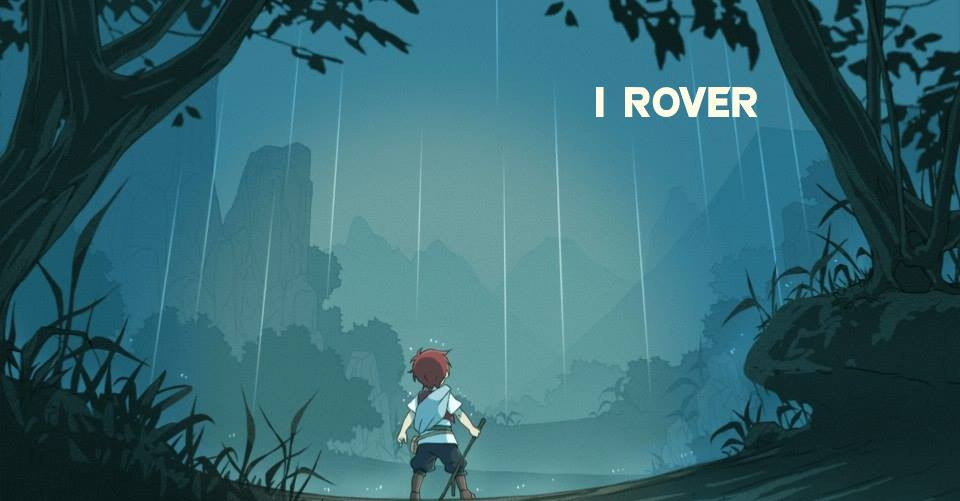
\includegraphics[width=350pt]{Illustration/proj_irover.jpg}
	\caption{iRover, l'histoire d'un héros qu'on appellait robot}
\end{figure}



\newpage


\renewcommand{\contentsname}{Sommaire} 
\tableofcontents

\newpage



\section{iRover, l'histoire d'un héros}

%background, histoire, scénario

\vspace{1cm}

Cette partie est dédiée à l'histoire de notre héros, son monde et ses motivations.
Si vous désirez en apprendre plus, laisser moi vous compter son histoire.

\vspace{1cm}

\subsection{Le monde de Lorr}

\vspace{1cm}

\begin{figure}[h]
	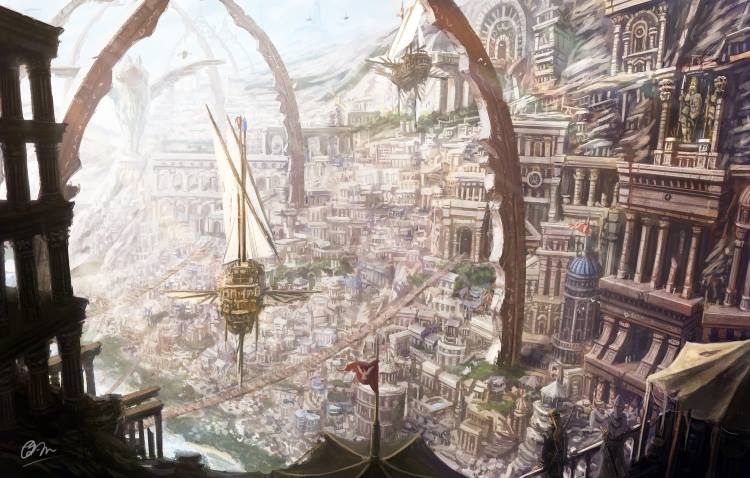
\includegraphics[width=350pt, height=180pt]{Illustration/Lina.jpg}
	\caption{Lina}
\end{figure}

\vspace{1cm}

Le pays de Lorr, vaste étendu de terre fertile entouré de montages et de forêts luxuriantes, abrite la vallée perdu du Vertou, 
là où nul n'a mit les pieds depuis plusieurs siècle.\\
On raconte que c'est ici que le grand pirate du nom de Stevy J. y aurait caché un trésors :"le chamalo magique".\\
Notre héros, intrépide aventurier du nom de Rover quitte alors sa ville natale Lina, où l'industrie et la maitrise de l'acier règne,  et part à la recherche de cette sucrerie antique.\\

\newpage

Cependant  cette mystérieuse vallée est habitée par d'étranges créatures : "des chou-kêtes".\\
Une horde de monstre farouchement attaché à leur territoire connu pour attaquer quiconque y pénetrera.\\

\vspace{1cm}

\begin{figure}[h]
	\includegraphics[width=350pt]{Illustration/vertou.jpg}
	\caption{Vertou}
\end{figure}



\vspace{1cm}


\newpage
\subsection{Stevy J.}

\vspace{1cm}

\begin{figure}[h]
  	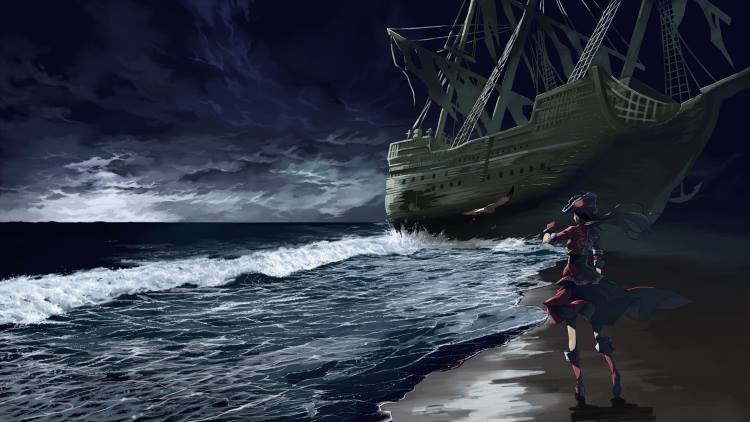
\includegraphics[width=350pt]{Illustration/Steve.jpg}
	\caption{Illustration du bateau de Steve}
\end{figure}

\vspace{1cm}

A une époque lointaine, Steven Joseph Obs de son nom complet, grand pirate et chasseur de trésor, écuma les 8 océans du monde pour venir finir ses jours dans le pays de Lorr.\\
On raconte qu'il aurait réussi à trouver le chamalo magique un artefact qui apporterait gloire, richesse et sucrerie infinie à quiconque le possèdera.\\
Stevy sera capturé et pendu pour piraterie et ne révèlera jamais ses secrets même dans sa biographie post mortem.\\
Beaucoup d'aventurié ont tenté de retrouver son trésor partout dans le monde mais il n'existe qu'un seul endroit où personne n'a mit les pied après le passage du celèbre pirate.



\newpage

\subsection{Rover, un héros pas comme les autres}

\vspace{1cm}

\begin{figure}[h]
  	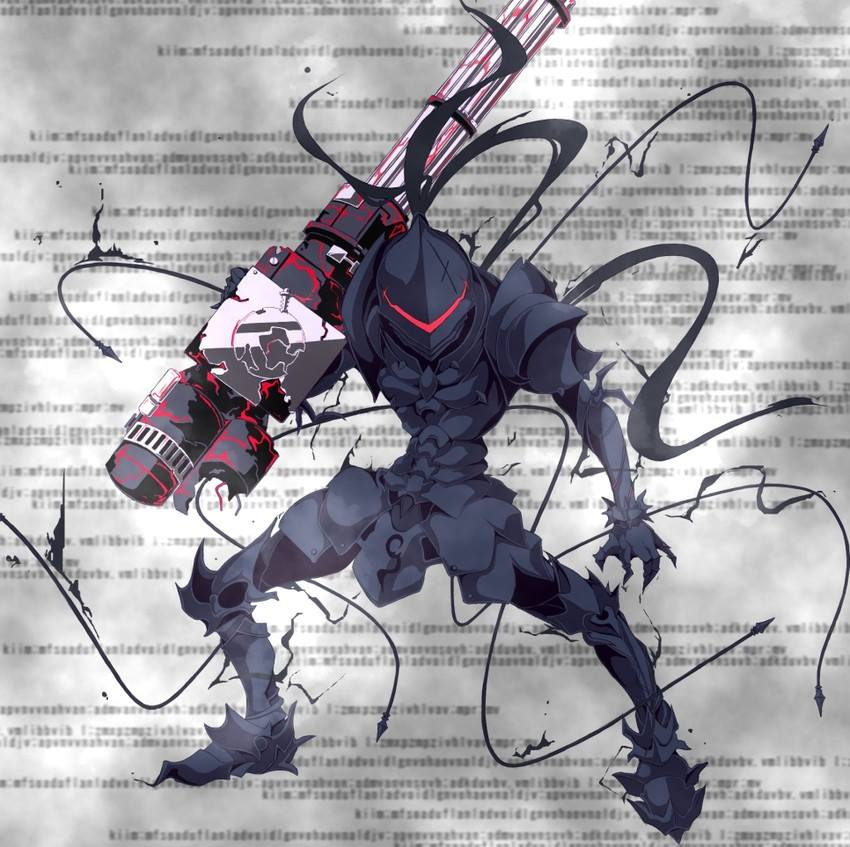
\includegraphics[width=350pt]{Illustration/Rover.jpg}
	\caption{Rover en Armure}
\end{figure}


Rover, notre héros, un apprenti forgerons reve d'aventure ! Ses années d'apprentissage lui permit de créer une armure lui donnant une apparance de robot et surtout augmentant sa protection contre les dangers de la vie au quotidient.
Lors de ses excursions il ne sort jamais sans son arme :  un petit bazooka, une arme de poing d'une très grande puissance.


\subsection{Les Chou-kêtes}
\vspace{1cm}


\begin{figure}[h]
  	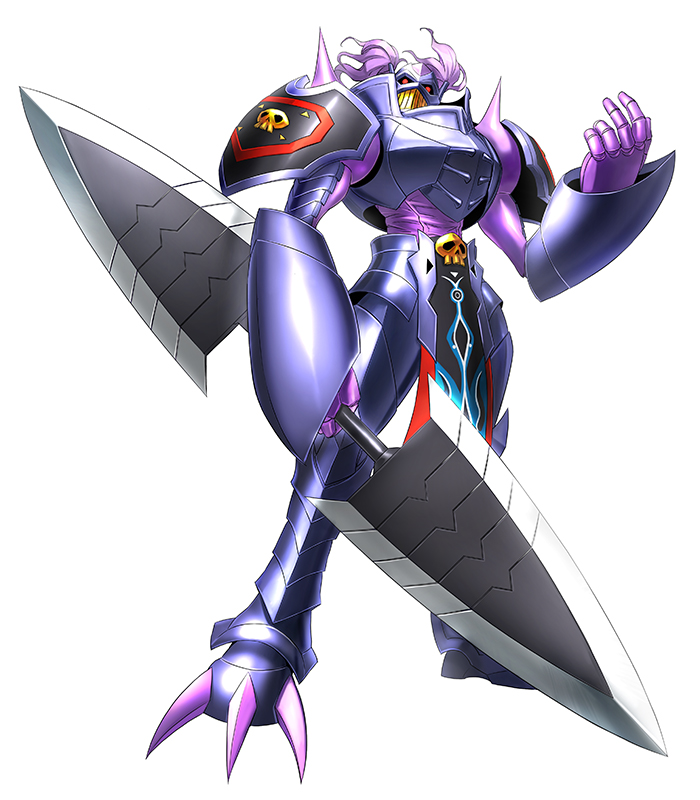
\includegraphics[width=300pt]{Illustration/Badboy.jpg}
	\caption{Général des Chou-Kêtes}
\end{figure}

\vspace{0.8 cm}

Bien des sciècles après la mort de Stevy J. On raconte que des créatures marines surgirent des océans pour venir habité dans la valée.
Personne ne sait exactement qui ils sont, d'ou ils viennent. Le dialogue avec ces êtres est impossible et il ne réponde que par la violence aux étrangers qui
pénetre sur leur territoire.



%regle du jeu

\section{But du jeu}


\vspace{2cm}

L'objectif principal du jeu (ou plutot de notre jeune amis) est de ramasser tous les trésors présents 
sur le terrain afin d'atteindre gloire et richesse et surtout un jour trouver le chamalo magique.\\

Des coffres seront disséminés sur la carte, souvent derrière des obstacles que le héros devra contourner.\\ 
Des ennemis (les chou-kêtes) pourront également attaquer notre héros et donc un combat sans merci s'enclanchera entre héros et monstre.\\


\begin{figure}[h]
   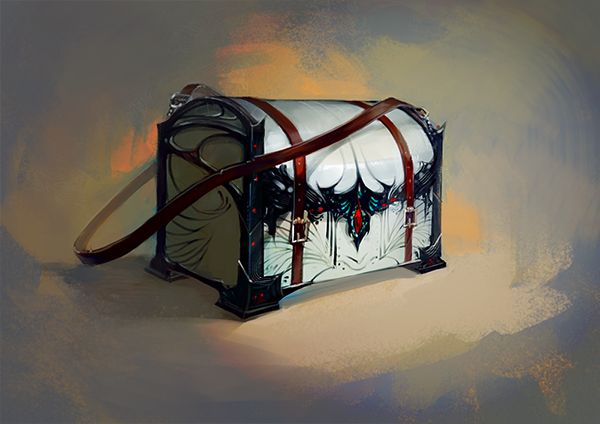
\includegraphics[width=350pt]{Illustration/coffre.jpg}
\caption{coffre au trésor}
\end{figure}


Le jeu prendra fin une fois tous les coffres ramassés ou si notre héros ne peut plus continuer son aventure.




\newpage

\section{Manuel d'installation}

\vspace{1.5cm}


\subsection{makefile}

%expliquer l'installation

%expliquer les librairies à utiliser
%parler de l'option pour que ça compile avec tout les systemes d'exploitation

\subsubsection{gestion des systeme d'exploitation}

\subsection{.config ????????}
%a virer si on utilise pas
%les options du makefile
%a ambélir si on a des idées (rappelle que meme si c'est pas implémenté, ça peut nous donner des points)


\newpage

\section{Documentation utilisateur}

%documentation utilisateur : donner des informations à des utilisateurs lambda sans grande connaissance informatique, avec des mots simple sur le fonctionnement de l'application.
%donner egalement une description simple de comment est faite ou est géré les partie de l'application.

\vspace{2cm}

Cette partie est dédiée aux utilisateurs recherchant à comprendre les méchanismes de cette petite application.
Si vous voulez des détails technique merci de vous referrez au Manuel Technique.
Nous vous expliquerons ici comment les divers élément du jeux s'articule afin de vous permettre une meilleur expérience utilisateur.

\vspace{0.5cm}	

\subsection{Les personnages}

\vspace{1cm}


Le jeu possède deux type de personnages : 

\vspace{0.5cm}

\begin{enumerate}
	\item Le héros, notre rover ou petit robot
	\item Les ennemis, les chou-kêtes.
\end{enumerate}

\vspace{0.5cm}

Ces deux types de personnage peuvent à la fois :

\vspace{0.5cm}

\begin{enumerate}
	\item se déplacer, avancer case par case 
	\item combattre, lancer un combat
\end{enumerate}

\vspace{0.5cm}

Chaque personnage possède des coordonnées indiquant leur emplacement en temps réel sur la carte ainsi que des statistiques propre à chacun mais aussi possèdera une armure ainsi qu'une arme.

\newpage
\subsubsection{Le robot, Rover}
\vspace{1cm}

Le robot se déplace sur la carte case par case et rencontrera des obstacles. \\
N'ayant pas appris à nager et du à des crises de vertiges récurente, il ne pourra ni se déplacer sur l'eau ni grimper sur les rochers,
les arbres, les murs et même les buissons !\\
Le robot, en plus de pouvoir se déplacer sur le terrain, peut aussi ramasser des clefs et ouvrir des coffres.\\
Pour celà, le robot possède un inventaire de clef représenter par le nombre de clefs que possède le robot.\\
Lorsque le robot va ramasser une clef, le nombre de clefs que le robot possède augmente donc de 1.\\
Inversement, lorsque notre robot ouvrira un coffre, le nombre de clefs dont il dispose diminura de 1 tout en sachant qu'il n'arrivera pas à ouvrir un coffre sans clef.\\
Le robot devra également combattre les ennemis pour rester en vie si il a le malheur de croiser un chou-kête.\\
Il possède une armure et une arme.
Le robot peut également prendre connaissance de ce qui l'entoure grâce à sa vision et ses senseurs. Il sait donc où aller et quoi faire.

\vspace{0.75cm}

\subsubsection{Les ennemis}


\vspace{0.75cm}


Certains ennemis seront présent sur le terrain et mettrons le robot en difficulté.\\ 
Le robot devra alors combattre ces ennemis s'il les rencontre afin de rester en vie.
Lorsque le robot se trouve à côté d'un ennemi, il est obligé de le combattre. 
Une fois l'ennemi vaincu, celui-ci disparait du terrain mais dans le cas contraire, notre héros ne sera plus en mesure de continuer et notre jeu prendra fin.\\
Les ennemis tout comme le héros peuvent se déplacer sur la carte mais ils auront un déplacement différent par rapport au héros.



\newpage
\subsection{Les coffres}


\vspace{0.75cm}

Les coffres sont des éléments posé aléatoirement sur la carte. Ils possèdent des trésors que notre héros souhaite récupérer.
Ils ne peuvent s'ouvrir qu'à l'aide de clefs.


\vspace{0.75cm}

\subsection{Les clefs}

\vspace{0.75cm}

Les clefs sont des éléments posé aléatoirement sur la carte. Ils permettent d'ouvrir les coffres au trésor disséminé un peu partout sur la carte.\\
Les clefs se détériore après leur utilisation fesant d'eux un consomable.


\vspace{0.75cm}


\subsection{L'environnement}


\vspace{0.75cm}

La carte sur laquelle le robot se déplace est constitué de cases comme appelles comunémant des Tiles (carreaux). \\
On distingue deux types de cases:

\begin{enumerate}
	\item Les cases où le robot peut se déplacer.
	\item Les cases où le robot ne peut pas se déplacer.
\end{enumerate}

Ces cases permette de décrire le décord et le type de terrain où se balade notre robot.
L'environement sert de base également pour la disposition des autres éléments tel que les coffres, les clefs, et ennemis.\\
La rencontre avec un de ces éléments entraine une gestion d'évênements.

\newpage
\subsection{La gestion des évênements}


\vspace{0.75cm}
Le robot, notre amis rover, devra faire face à beaucoup d'évênements, ouvrir un coffre, se battre contre un ennemi, ramasser une clef, se cogner contre un mur etc..
Tout ceci est géré par le comportement de chaque entité mais aussi pour l'affichage de l'environement.

Par exemple il doit être possible de marcher sur une clef pour la ramasser alors qu'il doit être impossible de marcher sur un ennemis

\vspace{0.75cm}

\subsubsection {Rencontre avec un ennemi}

\vspace{0.75cm}
 
Un ennemis et notre héros devront avoir la même importance physique : il ne peuvent pas se superposer.
Un ennemis et notre héros n'auront besoin que d'un regard pour enclanché le combat ! (1 case de différence )

%mettre un schéma
\vspace{0.75cm}

\subsubsection {Ouvrir un coffre}

\vspace{0.75cm}

Un coffre et notre héros n'ont pas la même importance physique : le héros devra pouvoir "marcher" sur le coffre.\\
Un coffre et notre héros devront impérativement être sur la même case pour que le coffre puisse s'ouvrir et ce dernier, le héros, devra avoir une clé pour que cela soit possible.

%mettre un schéma
\vspace{0.75cm}

\subsubsection {Ramasser une clé}

\vspace{0.75cm}
Une clé et notre héros n'ont pas la même importance physique : le héros devra pouvoir "marcher" sur la clé.
La clé et notre héros devront impérativement être sur la même case pour que la clé puisse être ramasser par ce dernier.
L'inventaire de clé augmentera alors.

%mettre un schéma
\vspace{0.75cm} 
\subsection{L'interface utilisateur}

\subsection{IA}

L'intelligence artificielle est dans notre application ce qui détermine le scénario de ce mini jeu.
En effet notre robot se déplace et agit de façon intelligente.
\vspace{0.75cm}

\subsubsection{Le Path Finding}

\vspace{0.75cm}

Le path finding correspond à la capacité du robot à trouver un chemin à suivre pour atteindre un objectif qu'il se fixe.
Par exemple : 

\vspace{0.5cm}

\begin{enumerate}
\item "Je dois retrouver mon amis qui est en bas à droite de la carte"
\item "Je suis au centre de la carte"
\item "Je regarde le chemin le plus simple pour y aller"
\item "Je le suis jusqu'à destination"
\end{enumerate}

\vspace{0.75cm}

\subsubsection{La découverte de la carte}

\vspace{0.75cm}

La découverte de la carte est ce qu'on appelle un senseur.
Meme si notre amis Rover est pixéliser il est doté de sens lui permettant de "voir" ce qui l'entour et de comprendre son environement.
Afin d'utiliser le path finding (expliqué au paragraphe précédent)
il a besoin de savoir où il est et où il doit se rendre.

\vspace{0.75cm}

\subsection{Les conditions de fin du jeu}

\vspace{0.75cm}

Le jeu se termine sous deux conditions bien distainct.
Soit le héros n'est plus apte à continuer son aventure après un combat.
Soit le héros a récupéré tout les coffres de la carte et a réussi son objectif.

\newpage

\section{tutoriel}

\end{document}


